\section{Sumador/restador \label{sec:s3}}

\begin{center}
	\begin{minipage}{12cm}
		\begin{tcolorbox}[title=Actividad 3]
			Codificar el sumador/restador presentado en la lámina 12 y verificar como se implementa utilizando el visor RTL.
		\end{tcolorbox}	
	\end{minipage}
\end{center}

La visualización RTL del sumador/restador en VHDL se muestra en la \autoref{fig:adder_subtractor_vhdl_rtl} y en Verilog en la \autoref{fig:adder_subtractor_verilog_rtl}. Como se observa, la implementación del sumador/restador se hace utilizando un multiplexor que selecciona la salida deseada con la variable C. Las simulaciones para el código en VHDL se visualizan en la \autoref{fig:adder_subtractor_vhdl_WaveBi} en base binaria y en la \autoref{fig:adder_subtractor_vhdl_WaveDe} en base decimal. En cambio, las simulaciones para el código en Verilog se visualizan en la \autoref{fig:adder_subtractor_verilog_WaveBi} en base binaria y en la \autoref{fig:adder_subtractor_verilog_WaveDe} en base decimal. Los valores empleados son los mismos que los de la Actividad 1.

\begin{figure}[ht]
	\centering
	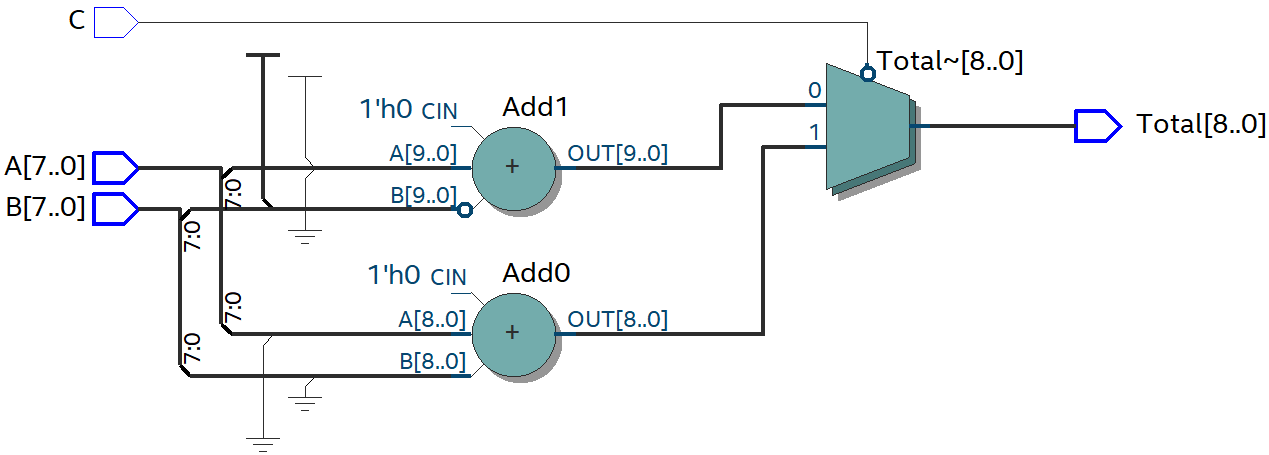
\includegraphics[scale=0.5]{Adder_Subtractor_VHDL_RTL.png}
	\caption{Diagrama RTL del sumador/restador en VHDL. \label{fig:adder_subtractor_vhdl_rtl}}
\end{figure}

\begin{figure}[ht]
	\centering
	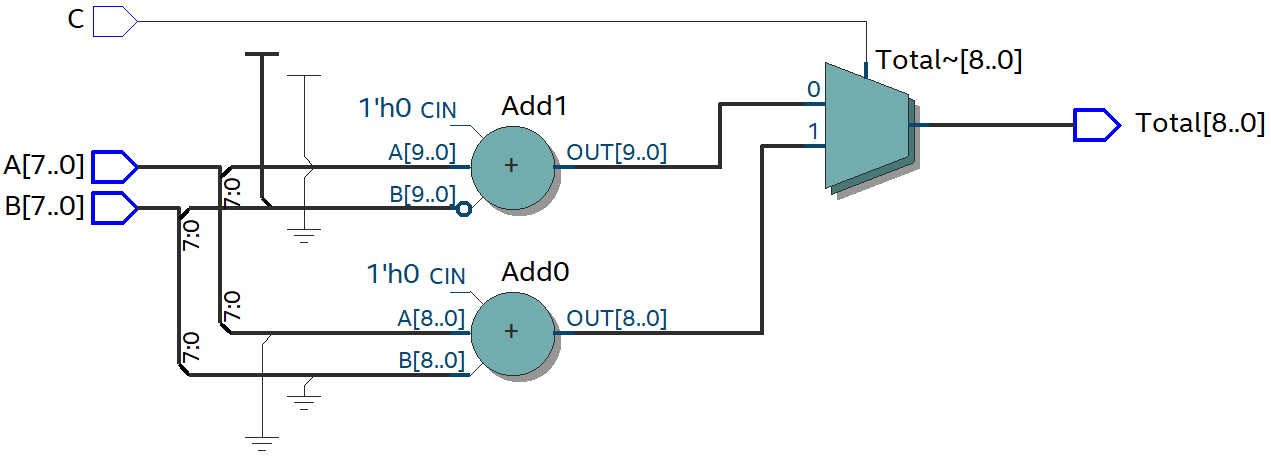
\includegraphics[scale=0.5]{Adder_Subtractor_Verilog_RTL.png}
	\caption{Diagrama RTL del sumador/restador en Verilog. \label{fig:adder_subtractor_verilog_rtl}}
\end{figure}

\begin{figure}[ht]
	\centering
	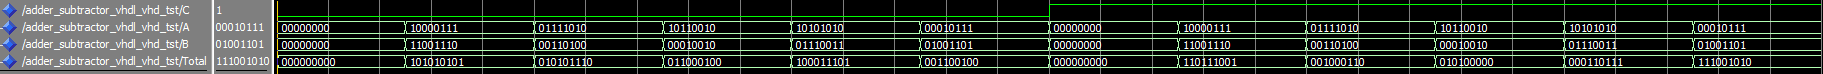
\includegraphics[scale=0.35]{Adder_Subtractor_VHDL_WaveBi.png}
	\caption{Simulación del sumador/restador en VHDL con el visor de formas de onda de ModelSim (Base binaria). \label{fig:adder_subtractor_vhdl_WaveBi}}
\end{figure}

\begin{figure}[ht]
	\centering
	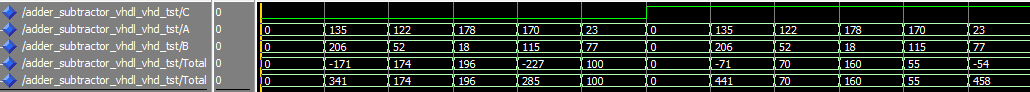
\includegraphics[scale=0.6]{Adder_Subtractor_VHDL_WaveDe.png}
	\caption{Simulación del sumador/restador en VHDL con el visor de formas de onda de ModelSim (Base decimal). \label{fig:adder_subtractor_vhdl_WaveDe}}
\end{figure}

\begin{figure}[ht]
	\centering
	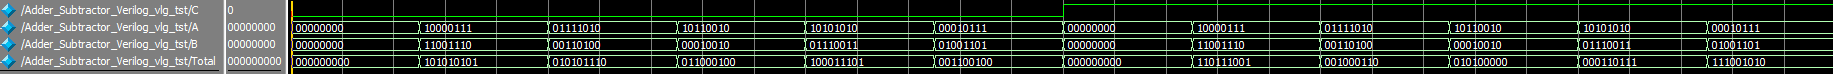
\includegraphics[scale=0.35]{Adder_Subtractor_Verilog_WaveBi.png}
	\caption{Simulación del sumador/restador en Verilog con el visor de formas de onda de ModelSim (Base binaria). \label{fig:adder_subtractor_verilog_WaveBi}}
\end{figure}

\begin{figure}[ht]
	\centering
	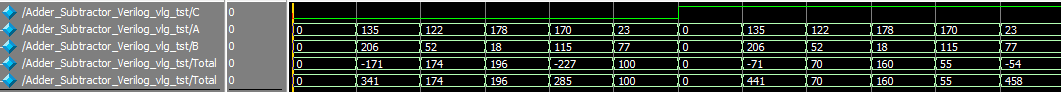
\includegraphics[scale=0.6]{Adder_Subtractor_Verilog_WaveDe.png}
	\caption{Simulación del sumador/restador en Verilog con el visor de formas de onda de ModelSim (Base decimal). \label{fig:adder_subtractor_verilog_WaveDe}}
\end{figure}